% !TEX root = CI_Adoption.tex

\section{Methods}
\label{sec:method}

We collected and statistically analyzed data from a sample of open-source 
Java (language chosen based on familiarity of the first author) projects on 
\GH, that adopted \Tvis at some point during their history.

\subsection{Data Gathering}

Data collection involved mining multiple sources, the \GH API, project version 
control (git) logs, and the \Tvis API.
The goal was to select non-trivial projects that adopted \Tvis, and had sufficient
activity both before and after adoption, in order to observe potential transition effects.
Note that for the purpose of this study we don't distinguish between ``project'' 
and ``repository''; the term ``project'' has also been used to refer to a collection 
of interrelated repositories in the literature~\cite{vasilescu2016sky}.

We started by composing (using the \GH Search API) a list of candidate Java 
projects that: (i)~were not very small (a large fraction of projects on \GH are 
small and inactive~\cite{gousios2014exploratory}; we arbitrarily chose to ignore
projects smaller than 500 kilobytes, using the \GH Search API's \emph{size} 
parameter); and (ii)~were created no later than 2014-11-08. 
The second criterion is a consequence of our data collection date (2016-05-01)
and the ``sufficient history'' requirement. 
Our statistical analysis, detailed below, assumes 9 months of history for each
project both prior to and after adopting \Tvis; since we did not have access to
data on when each project started using \Tvis at this stage, we conservatively
chose the 2014-11-08 date, which allows 9*30*2 days of history from project 
creation to 2016-05-01.
This step resulted in a list of over 300,000 candidate Java projects.

%first and foremost, we should make sure our studied projects have sufficient history (e.g. 9*30 days) both before using Travis-CI and after using Travis-CI.  As the data were extracted from the inception until 2016-05-01, the projects selected should be created at least before 2014-11-08, so that there are at least 9*30*2 days from its creation to 2016-05-01. 
%From GitHub Search API, we first found over 300k Java projects created before 2014-11-08 and with $\geqslant 500$ kilobytes. 
%After consulting Travis-CI, we further identify projects that: 1) adopted Travis-CI; 2) at least 9 * 30 days from project creation to Travis-CI adoption; 3) at least 9 * 30 days from Travis-CI adoption to 2016-05-01. This filtering process left us 1566 projects.  
%For each project, we collect the whole history of commits, issues, and pull requests from GitHub API, and the history of Travis-CI builds and job logs from Travis-CI repository using the ruby library of \textit{travis gem}.  In addition to these publicly available data, we further gathered the information about the number of tests and types of errors during the Travis-CI run.

Next, we used the \Tvis API to determine which of these projects:
(i)~used \Tvis, and if yes, we recorded the date of the earliest build as the 
adoption date; (ii)~had at least 9*30 days of history from project creation to 
the adoption date, and from the adoption date to 2016-05-01, respectively. 
This filtering process resulted in 1,566 projects.
For each project, we collected: (i)~its history of commits, issues, and pull 
requests using the \GH API; and (ii)~its history of \Tvis builds and, for each
build, all its job logs (a \Tvis build can be configured to run multiple jobs,
one for each set of user-defined configuration options; each job run produces 
a ``build log''), using the \Tvis API and the \textit{travis gem} Ruby library.  
In addition to these publicly available data, we parsed the build logs and 
further extracted information about the number of tests executed and the 
types of reasons causing builds to break.
We provide more details next.

% !TEX root = ../CI_Adoption.tex

\begin{table}[t] \centering
\small
  \caption{Examples for the outputs in terms of MAVEN, GRADLE and ANT
  \vspace{-0.2cm}
  }
  \label{log_example}

\begin{tabular}{ p{8cm}}
	\hline
	\\[-1.8ex]\hline
		\textbf{MAVEN}         \\
		\begin{tabular}[c]{@{}l@{}}
			\textit{-------------------------------------------------------}\\ 
			\textit{ T E S T S}\\ \textit{-------------------------------------------------------}\\ 
			\textit{Running org.sonar.ide.intellij.inspection.InspectionUtilsTest}\\ \textit{Tests run: 1, Failures: 0, Errors: 0, Skipped: 0, Time elapsed:}\\ \textit{0.202 sec}\\ 
			\textit{Results:}\\ 
			\textit{Tests run: 1, Failures: 0,Errors: 0, Skipped: 0}\end{tabular} \\  \hline
	
		\textbf{ANT}          \\
		\begin{tabular}[c]{@{}l@{}}
			\textit{{[}junit{]} Running limelight.BufferedImagePoolTest}\\ 
			\textit{{[}junit{]} Testsuite: limelight.BufferedImagePoolTest}\\ \textit{{[}junit{]} Tests run: 5, Failures: 0, Errors:0, Time elapsed: 0.143 sec}\end{tabular}                                                                                                                                                \\  \hline
		\textbf{GRADLE}          \\
		\begin{tabular}[c]{@{}l@{}}
			\textit{:test}\\ 
			\textit{...}\\ 
			\textit{1 test completed, 1 failed}\\
			\textit{:test FAILED}\\ 
			\textit{Total time: 3.8 secs}\end{tabular}      \\ \hline                                                                                                                                                                                                                                                
	\end{tabular}
\end{table}

\smallskip\noindent\emph{Number of tests executed per build:} 

Each \Tvis build consists of at least one job, which corresponds to a particular
build \& test environment (\eg jdk version, environment variables). 
Once the job is started, a log is generated, recording the detailed information
of the build lifecycle, including installation steps and output produced by the 
build managers. % scripts for testing. 
Figure~\ref{log_example} shows fragments of the logs generated by the 
three widely used Java build tools, Maven, Ant, and Gradle. 
To investigate the evolution in testing practices across builds, we wrote a tool 
to analyze the logs and extract summary information about test executions.  
Since the relationship between builds and jobs is one-to-many, we use the 
maximum number of tests across jobs as the test count for the build. 

% !TEX root = CI_Adoption.tex

\begin{table}[t] \centering
\small
  \caption{Travis-CI build failure taxonomy
  \vspace{-0.2cm}
  }
  \label{error_types}

\begin{tabular}{ p{1.5cm}  p{2.5cm}  p{4cm} }
	
\hline 
\\[-1.8ex]\hline
Category & Description & Examples of textual patterns \\ \hline 
\emph{failed test} & tests were failed & tests failed, TestsFailedException, tests unsuccessful\\ \hline
\emph{skipped or pending test} & tests were skipped or set to be pending & skipped tests \\ \hline
\emph{missing file or dependency} & required files or dependencies are not available &  FileNotFoundException, no such file to load, is not installed \\ \hline
\emph{code quality} & the code failed to satisfy the code standards & line too long, missing whitespace around operator, too many pylint violations \\ \hline
\emph{compile error} &compilation errors happened & Compilation failed, syntax check failed, attributeError, parse error\\ \hline
\emph{execution error} &an error occurs during the execution of code & runtime error, execution failed, test errors, OutOfMemoryError\\ \hline
\emph{time out} & the build could not be completed within the required time&“test run exceeded * minutes”, “..took longer than”, command time-out \\ \hline 
\emph{other} &other infrequent errors are included in this type & warnings on documentation, Aborted due to warnings, The remote end hung up unexpectedly \\
\hline

\end{tabular}

\end{table}



\smallskip\noindent\emph{Error classification for failed builds:}

\Tvis marks a build as \textit{failed} if at least one of its jobs not explicitly 
labeled as \emph{allowed to fail} in the project's CI configuration 
file\footnote{\url{https://docs.travis-ci.com/user/customizing-the-build/#Rows-that-are-Allowed-to-Fail}} failed.
Therefore, to understand why \Tvis builds failed, we proceed to find out 
what happened in the jobs. 
We first manually reviewed a set of failed jobs to recognize what kinds of 
failures occur and whether there are any corresponding textual patterns in 
the logs. 
Then, we extracted a group of mapping rules to classify these patterns into 
categories. 
To mitigate the risk of bias arising from missing and incorrect classification, 
we augmented the manual reviewing rates to improve our classification 
rules and remove spurious classification as much as possible. 
The classification scheme evolved over the process of manual review, and 
was gradually refined to cover more textual patterns. 
In the end, we identified 8 categories of reasons for build failures, 
as summarized in Table~\ref{error_types}. 
%a group of mapping rules to classify the errors into 8 types, as shown 

Next, we implemented tools to perform the classification automatically. 
The detailed process consists of the following steps: 1)~\emph{Failure Location}. 
We first recognized failed jobs with \textit{non-allow-failure} attributes, which 
result in the build's final \textit{failed} state. 
Then, we attempted to locate the command which caused the breakdown 
in the log file, as the command which exited with a non-zero value.
The log entry for this command usually provided detailed information about 
the fatal errors that occurred. 
If such commands were not recorded in the log file, we expanded the search 
scope to the \textit{script} phase and the \textit{after script} phase of the 
build log, as per \Tvis build lifecycle.\footnote{\url{https://docs.travis-ci.com/user/customizing-the-build/#The-Build-Lifecycle}}
Note that if errors occur in the \emph{before script} phase of the build, the 
job is automatically marked as \textit{errored} and stops immediately. 
Only if the \textit{script} phase returns a non-zero exit code, or the \textit{after 
script} phase times out, then the job is marked as \textit{failed}. 
Therefore, we first check if there is a time-out error in \textit{after script}. 
If not, then it's likely that the errors in the \textit{script} phase caused the 
build to break. 
2)~\emph{Log Parsing}. 
After extracting the log fragment that described which errors occurred, we 
used textual pattern matching to classify the errors. 
3)~\emph{Classification}. 
After extracting the textual patterns, we categorized them into the defined 
8 types based on the rules. 
Note that there is a one-to-many relationship between jobs and failure types. 
For example, if a job had both failed tests and skipped tests, it is tagged 
with both ``failed test'' and ``skipped or pending test'' types.


%\textit{Distinguishing the bugs introduced before CI adoption and the bugs introduced after CI adoption}: 
%We suppose that the defects before and after introducing Travis-CI are different. To verify this, we use the SZZ algorithm to gather bug data, and divide them into two groups ( \ie bugs introduced before Travis-C and bugs introduced after Travis-CI ).
%In GitHub, when a bug is reported, an issue will be created to track this bug, and subsequently a set of commits occur for bug fixing. 
%We decide whether a issue is a \textit{fix issue} based on the constrains that 1) the issue has been taged as a bug (with labels like \textit{bug}, \textit{defect}, \textit{fault}); 2) the issue has at least one commit with source file modification to fix this bug. To do this, We first analyze the commit messages to recognize its corresponding issue based on the special textual patterns (\eg fix \textit{issue\_id}, close \textit{issue\_id}, gh-\textit{issue\_id}), and then check if this issue has bug tag. If yes, we will use git diff to find the change details (\ie changed files and lines), and further check if the commit has changed source files.
%After the above conditions checking, we identify fix issues and the corresponding fix commits. The lines changed in fix commits are targeted to fix the bug. Using \textit{git blame}, we can locate which commit last added or modified these lines. We consider this commit as a buggy commit as it introduced bug. 
%As we know, a fix issue will only be triggered by the bug introduced before the issue is opened. Therefore, a necessary condition for filtering is that the buggy commit must have been pushed before the bug being reported (\ie issue being created), otherwise, this buggy commit should not be implicated.
%With above process, the bugs can be divided into two groups based on when the bugs were introduced (\ie buggy commit time) and when the project started using Travis-C. For each group, we gathered the bug logs from the fix issues and fix commits, and then built word cloud to analyze the differences between them.

%\subsection{Overview of the Data Set}
\subsection{Additional RQ-Specific Filtering}
\label{sec:dd}

% !TEX root = CI_Adoption.tex



\begin{table}[]
	\centering
	\caption{Summary statistics for 1566 studied projects}
	\label{projs_summary}
	\begin{tabular}{ p{1.2cm} p{0.7cm} p{0.7cm} p{0.7cm} p{0.7cm} p{0.7cm} p{0.7cm}}
		\hline
		Statistic       & Min            & 1st Qu.        & Median          & Mean           & 3rd Qu.        & Max             \\ \hline
		
		created\_at     & 2008/6/6 & 2011/8/8  & 2012/7/30 & 2012/6/27 & 2013/6/6  & 2014/11/7 \\
		size            & 500            & 1594           & 6006            & 40460          & 26980          & 2433000         \\
		
		\# stars        & 0              & 6              & 33.5            & 344.1          & 180.8          & 18480           \\
		\# forks        & 0              & 4              & 18              & 133.2          & 74             & 7247            \\
		
		\# commits      & 5              & 184.2          & 412             & 1385           & 1085           & 118000          \\
		\# issues       & 0              & 2              & 20              & 125.9          & 89.75          & 10330           \\
		
		\# PRs & 0              & 2              & 14              & 97.68          & 64             & 7715            \\
		\# builds       & 1              & 39             & 99.5            & 347            & 278            & 16700          
	\end{tabular}
\end{table}


%Our study makes use of a large-scale data set collected from the selected 1566 java projects. 
Table~\ref{projs_summary} contains descriptive statistics for the selected 
1,566 Java projects that adopted \Tvis. 
We note an average number of 347 builds per project. 
We further census the builds in terms of the event type and final state. 
Table~\ref{builds_count} shows that there are a total of 541,959 builds in 
our data set, 68\% coming from push commits and 32\% come from pull 
requests (PRs). 
Of these builds, 67.1\% were passed, 18.6\% were failed, and the others 
were errored or canceled. 
Besides, Table~\ref{count_info} lists the statistics for \#commits, \#issues 
and \#PRs before and after adopting \Tvis, respectively. 
We can preliminarily see that, in our studied projects, there are less commits 
after CI adoption, but more issues and PRs. 
From the summary statistics, we found there are large variances between 
projects in terms of each attribute, as shown in Table~\ref{projs_summary}. 
For example, 18\% of projects have a value of \#issues equal to 0, as they 
haven't featured \GH issue tracking yet. 
When studying the evolution practices of issues, these projects without 
issues may bias our conclusions. 
As a result, to avoid too many zeros in our subsequent time series analysis, 
we did more data filtering on the 1,566 projects for each RQ individually, 
based on different conditions as follows.

For RQ1 and RQ2, we study the code churn and commit frequency. 
In our data set, 8.9\% of commits are merge commits. 
First, we remove these merge commits, to avoid double counting and since 
they were automatically generated. 
Then, we further filter the projects based on the number of non-merge commits,
to reduce potential bias due to data sparsity (since we aggregate data at 
monthly intervals), and discard projects with less than 500 total non-merge 
commits.
%We Each project should have at least 500 nonmerge commits. 
In the end, the data set for RQ1 and RQ2 consists of 567 projects, with a 
total if 1,629,090 no-nmerge commits.

For RQ3, we only selected projects with at least 100 issues for similar sparsity 
avoidance reasons. 
The resulting filtered data set consists of 293 projects, with a total of 143,573 
\GH issues.

For RQ4, we investigate the changes in \#tests per build.
As introduced above, we collected \#tests from build logs. 
Again, as above, we first filtered the projects based on the number of builds
(lower bound arbitrarily set at 100), leaving 736 projects. 
%Each projects should have at least 100 builds. This selection left us 736 projects. 
Furthermore, during the collection of \#tests, we found (and subsequently
filtered out) 219 projects that did not execute any tests as part of their \Tvis 
builds, and additional 267 projects that tested very scarcely (\ie we kept 
projects for which at least 90\% builds executed at least one test). 
%We just removed these projects as they didn't have \# test values. 
In the end, the filtered data set for RQ4 consisted of 250 projects.
%Among the other projects, 250 of them have more than 90\% builds with at least one test. Here, we only consider these 250 projects with high coverage of testing ( \textgreater{ 90\%} ).

\subsection{Time Series Analysis Method}

We use data visualization and statistical modeling methods to discover 
longitudinal patterns indicative of CI adoption effects on development practices.
As one of the contributions of this paper, we introduce the statistical modeling 
framework of \emph{regression discontinuity design}~\cite{Imbens2008611} to assess the existence 
and extent of a longitudinal effect of CI adoption on development practices.

To evaluate the effect of a treatment, \eg a new drug on a disease progression, 
randomized experimental trials are typically used, in which the experimental 
cohort is randomly split into a treatment group, \ie those given the drug, and 
a control group, \ie those given an experientially identical placebo. 
Then, the effect is evaluated based on the difference in disease progression 
between the two groups.
In the absence of randomized trials, as is the case with the trace data that is
common in empirical software engineering, weaker techniques which make 
additional assumptions, \eg quasi-experiments, are employed.

Regression discontinuity design (RDD)~\cite{Imbens2008611} is an example of such a technique, 
used for modeling the extent of a discontinuity of a function between its values 
at points just before and just after a given intervention point. 
It is based on the assumption that in the absence of the intervention, the 
trend of the function would be continuous.
A common situation where a discontinuity occurs is illustrated in Fig.~\ref{RDDIllustration}, 
where the discontinuity is shown as occurring at the time of the intervention, 
and is manifested as a different regression before and after that point.

There are a number of different formalizations of RDD, most prominently 
sharp RDD and fuzzy RDD~\cite{imbens2008regression}.
Each, in turn, can be implemented in a variety of ways.
To model the effect of CI adoption on developer practices, here we chose one 
of the simpler approaches, namely linear regression with an interaction term.
We summarize our approach next, following the description from a survey for practitioners article by Imbens and Lemieux~\cite{imbens2008}.
We refer to Figure~\ref{RDDIllustration} for an illustration.
Let $Y$ be the outcome variable in which we are looking for a discontinuity, 
\eg commit churn per month, let $X$ be the temporal variable containing the 
time of intervention, and let $c$ be the time point at which the intervention, in 
this case CI adoption, has happened.
Then, an RDD model for points $x_i$ in equal intervals $h$ on each side of 
$c$, $c-h \le x_i \le c+h$, is given by:

\[y_i \ = \alpha + \beta(x_i-c) + \gamma w_i + \delta(x_i-c)w_i + \epsilon_i,\]

\noindent where $w_i = (x_i > c)$, \ie $w_i$ is 1 if point $x_i$ is included in 
the treatment group (\eg after CI adoption), and 0 if it is before the treatment.
In fact, this model encapsulates two separate regressions.
For points before the treatment, the resulting regression line has a slope of 
$\beta$, and after the treatment $\beta + \delta$.
The size of the effect of the treatment is the difference between the two 
regression values of $y_i$ evaluated at $x=c$, and can be seen to be equal 
to $\gamma$.
For example, in Fig.~\ref{RDDIllustration}, the treatment effect ($\gamma$) is negative, and there is an interaction effect ($\delta ne 0$) which changes the slope of the regression after the treatment.

For each project, we use an RDD model implemented as the above 
double linear regression, on data centered at the time of CI adoption, and 
having equal number of points on each side.
Solving the regression gives us the coefficients, which if significant, can help us reason about the treatment and its effects, if any.
 

\begin{figure}[t]
	\centering
	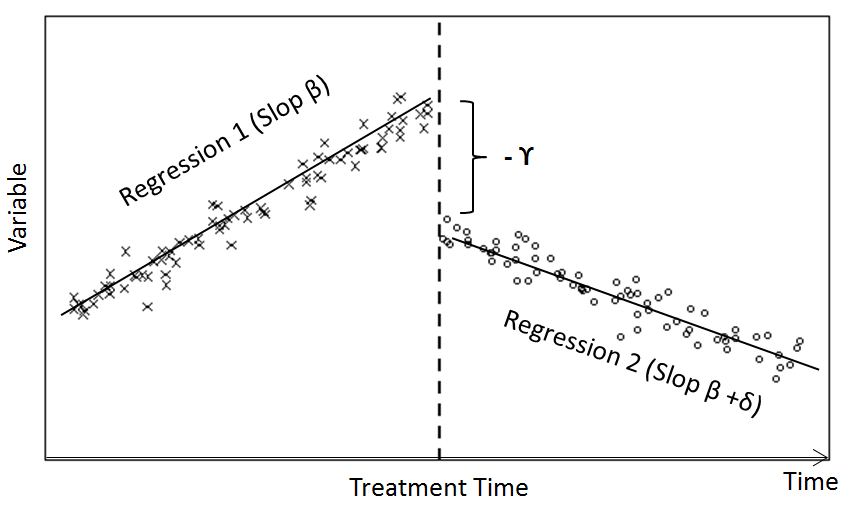
\includegraphics[width=0.5\textwidth, clip=true, trim=0 15 15 50]{RDD_ok.png}
	\caption{RDD Illustration}
	\label{RDDIllustration}
\end{figure}

